%%%%% This is a LaTeX file for an A3 poster.
%
%%%%%%%%%%%%%%%%%%%%%%%%%%%%%%%%%%%%%%%%%%%%%%%%%%%%%%%%%%%%%%%%%%%%%%%%%%%%%

%%%%%%%%%%%%%%%%%%%%%%%%%%%%%%%%%%%%%%%%%%%%%%%%%%%%%%%%%%%%%%%%%%%%%%%%%%%%%
%%%%%%%%%%%%%%%%%%%%%%%%%%%%%%%%%%%%%%%%%%%%%%%%%%%%%%%%%%%%%%%%%%%%%%%%%%%%%%
%%%%%%%%%%%%%%%%%%%%%%%%%%%%%%%%%%%%%%%%%%%%%%%%%%%%%%%%%%%%%%%%%%%%%%%%%%%%%

%%%%%%%%%%%%%%%%%%%%%%%%%%%%%%%%%%%%%%%%%%%%%%%%%%%%%%%%%%%%%%%%%%%%%%%%%%%%%
\documentclass{a0poster}
% To modify the size of the page:
\usepackage[dvips,centering,margin=1cm]{geometry}
\usepackage{multicol}
\usepackage[utf8]{inputenc}
\usepackage{color}

%%\renewcommand{\labelitemii}{$\star$}

\usepackage{amsmath, amsthm, amsfonts}
\newtheorem{lemma}{Lemma}
\newtheorem{sublemma}{Lemma}[lemma]
\usepackage{enumerate}
\usepackage{enumitem}
\usepackage{graphicx}           % Include figure files.
%\usepackage{titlesec}                  % Include figure files.
%\titlespacing*{\section}
%{0pt}{5.5ex plus 1ex minus .2ex}{4.3ex plus .2ex}
\usepackage{tikz}
\usetikzlibrary{decorations.markings,arrows,calc}
\usepackage{subcaption}

% Colors
% -------
\definecolor{azulillo}{rgb}{0.8,0.85,1}
\definecolor{marronrp3}{rgb}{.9,.9,.7}
\definecolor{salmon}{rgb}{1,.9,.8}
\definecolor{rojo}{rgb}{.6,.1,0}

\pagestyle{empty}

\def\to{\rightarrow}

% Hyphenation
%\hyphenation{coa-gu-la-tion frag-men-ta-tion}

% ===========================================================================

\title{}
\author{}
\date{}
\begin{document}
%\maketitle

\begin{center}
  \begin{minipage}{.19\linewidth}
  \begin{minipage}{.36\textwidth}
      \centering
        
\includegraphics[width=.7\textwidth,height=.8\textwidth,scale=1]{Poster/images/uh_red.png}\\
        \vspace{2.5cm}
        
\includegraphics[width=1\textwidth,height=.4\textwidth,scale=1.3]{Poster/images/UHD_logo.png}
  \vspace{-1.5cm}
  \end{minipage}
  \begin{minipage}{1\linewidth}
  \begin{minipage}{.5\textwidth}
      \begin{center}
        
\includegraphics[width=.85\textwidth,scale=1]{Poster/images/uhcl.png}
        %\vspace{-1.5cm}
        
\includegraphics[width=.85\textwidth,height=.3\textwidth,scale=1.2]{Poster/images/UHV-letters-only-min-500x168.png}\\
      \end{center}
  \end{minipage}
    \end{minipage}
 \end{minipage}
  %&
  \begin{minipage}{.6\linewidth}
    \begin{center}
      \Huge \textbf{Rate of Penetration Prediction Using Machine Learning Models}
      
      \normalsize \begin{center} %
      \setlength{\tabcolsep}{45pt} % Default value: 6pt
      \begin{tabular}{cccc}
           \textbf{MJ D Asuncion}        & \textbf{Dalton Carter }                & \textbf{Gopika Kizhuvettil}            & \textbf{Taven Tran}\\
       University of Houston-Downtown    &    University of Houston - Victoria    &    University of Houston-Clear Lake    &    University of Houston\\
       mjasuncion@acm.org                & daltocarter@outlook.com                & gopika751@gmail.com                    & taventran@gmail.com\\
      \end{tabular}\\
      \vspace{1cm}
      \begin{tabular}{cccc}
          &\textbf{Dvijesh Shastri PhD } & \textbf{  Kalyan Venugupal PhD} & \\
            & University of Houston-Downtown & Industry Professional & \\
           & shastrid@uhd.edu & kalyan100673@gmail.com &
      \end{tabular} 
     \end{center} 
    \end{center}
  \end{minipage}
  %&
  \hspace{.03\linewidth}
  \begin{minipage}{0.16\linewidth}
    \begin{center}
      
\includegraphics[width=.6\linewidth]{images/nsf-logo.png}
    \end{center}
  \end{minipage}
\end{center}

\vspace{-.7cm}

% ---------------------------------------------------------------------------
%\fcolorbox{black}{salmon}{
\begin{minipage}[t]{.96\textwidth}
\begin{center}
\noindent
\vspace{-.55cm}
\section*{Abstract}
\end{center}
\vspace{-.85cm}
{\large The success of drilling a well for geothermal, oil, and gas purposes are quantified by how quickly the desired depth is reached. The progress of a drilling operation is determined by the drill bits rate of penetration (ROP). In our research we use machine learning models to make the drilling process more efficient by predicting the ROP considering the  weight on bit (WOB), revolutions per minute (RPM), surface torque, and flow rate. Using data from \cite{oedi_1111}, we cleaned, integrated, and performed exploratory data analysis to train regression models that we evaluated and improved. We concluded that the model best applicable is Random Forest because of its efficiency in training time, memory consumption, and simplicity.}

\end{minipage}
%}

\setlength{\columnsep}{.5cm}
\begin{multicols}{3}


%\colorbox{marronrp3}{
%\vspace{-10cm} 
\begin{minipage}[t]{.90\linewidth}
\vspace{-.85cm}
\begin{center}
    \vspace{.05cm}
    \section*{Motivation}
\end{center}
\vspace{-.35cm}
\begin{itemize}
    \item {\large Optimize ROP prediction}
    \begin{itemize}
        \item {\large Train machine learning models to predict ROP in drilling operations}  
    \end{itemize}
    \item {\large Decide the best model to deploy}
    \vspace{-.2cm}
    \begin{multicols}{2}
    \begin{itemize}
        \item {\large Highest score values}
%        \item Ease of explanation
        %\item {\large Scalability}
        \item {\large Least computational time}
        %\item {\large Least training time}
    \end{itemize}
    \end{multicols}
\end{itemize}
\vspace{-.85cm}
%\end{minipage}
%}
\begin{center}
\noindent
\vspace{-.55cm}
 \section*{Correlation Analysis}
 \end{center}
 
%\vspace{.1cm}
\begin{flushright}
  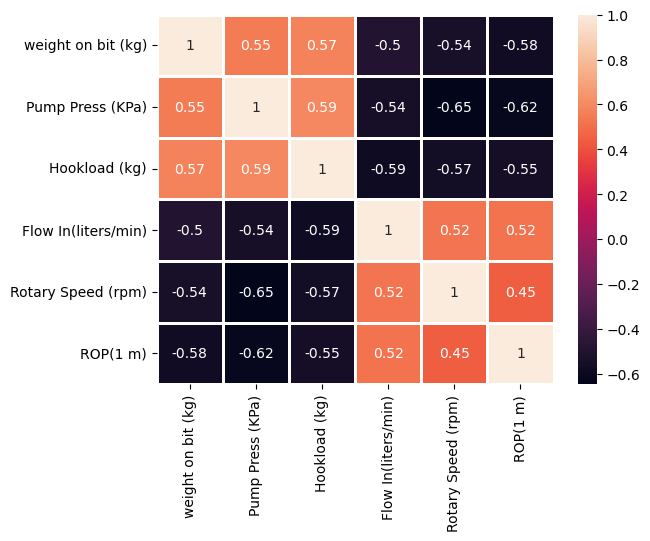
\includegraphics[width=1\textwidth, height=.70\textwidth, scale=1]{Poster/images/annotations.png}
%\vspace{.05cm}
\end{flushright}

\begin{center}
\noindent
\vspace{-.55cm}
\section*{Log Transformation}
\end{center}

\begin{center}
\begin{minipage}{.48\linewidth}
  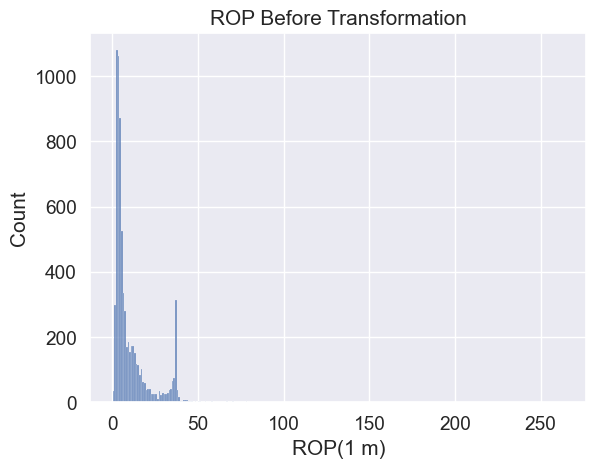
\includegraphics[width=1\linewidth, height=0.9\textwidth, scale=1]{Poster/images/Before.png}
\end{minipage}
\begin{minipage}{.48\linewidth}
  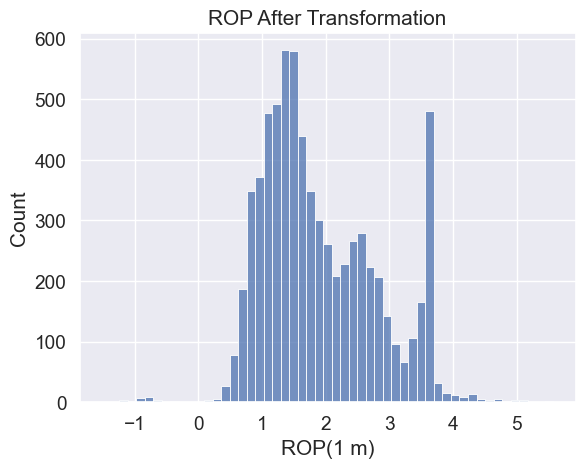
\includegraphics[width=1\linewidth, height=0.9\textwidth, scale=1]{Poster/images/After.png}
\end{minipage}  
\end{center}

%\vspace{-.40cm}
%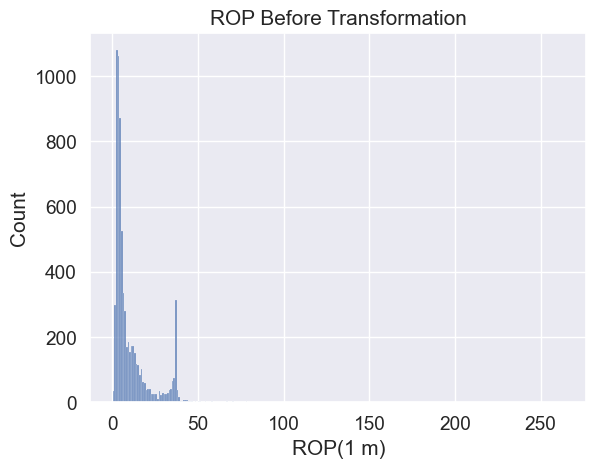
\includegraphics[width=.5\textwidth, height=.5\textwidth, scale=1]{Poster/images/Before.png}
\end{minipage}

%\vspace{-1.0cm}
\noindent
\begin{minipage}[t]{.96\linewidth}
    \vspace{-.5cm}
    \begin{flushright}
      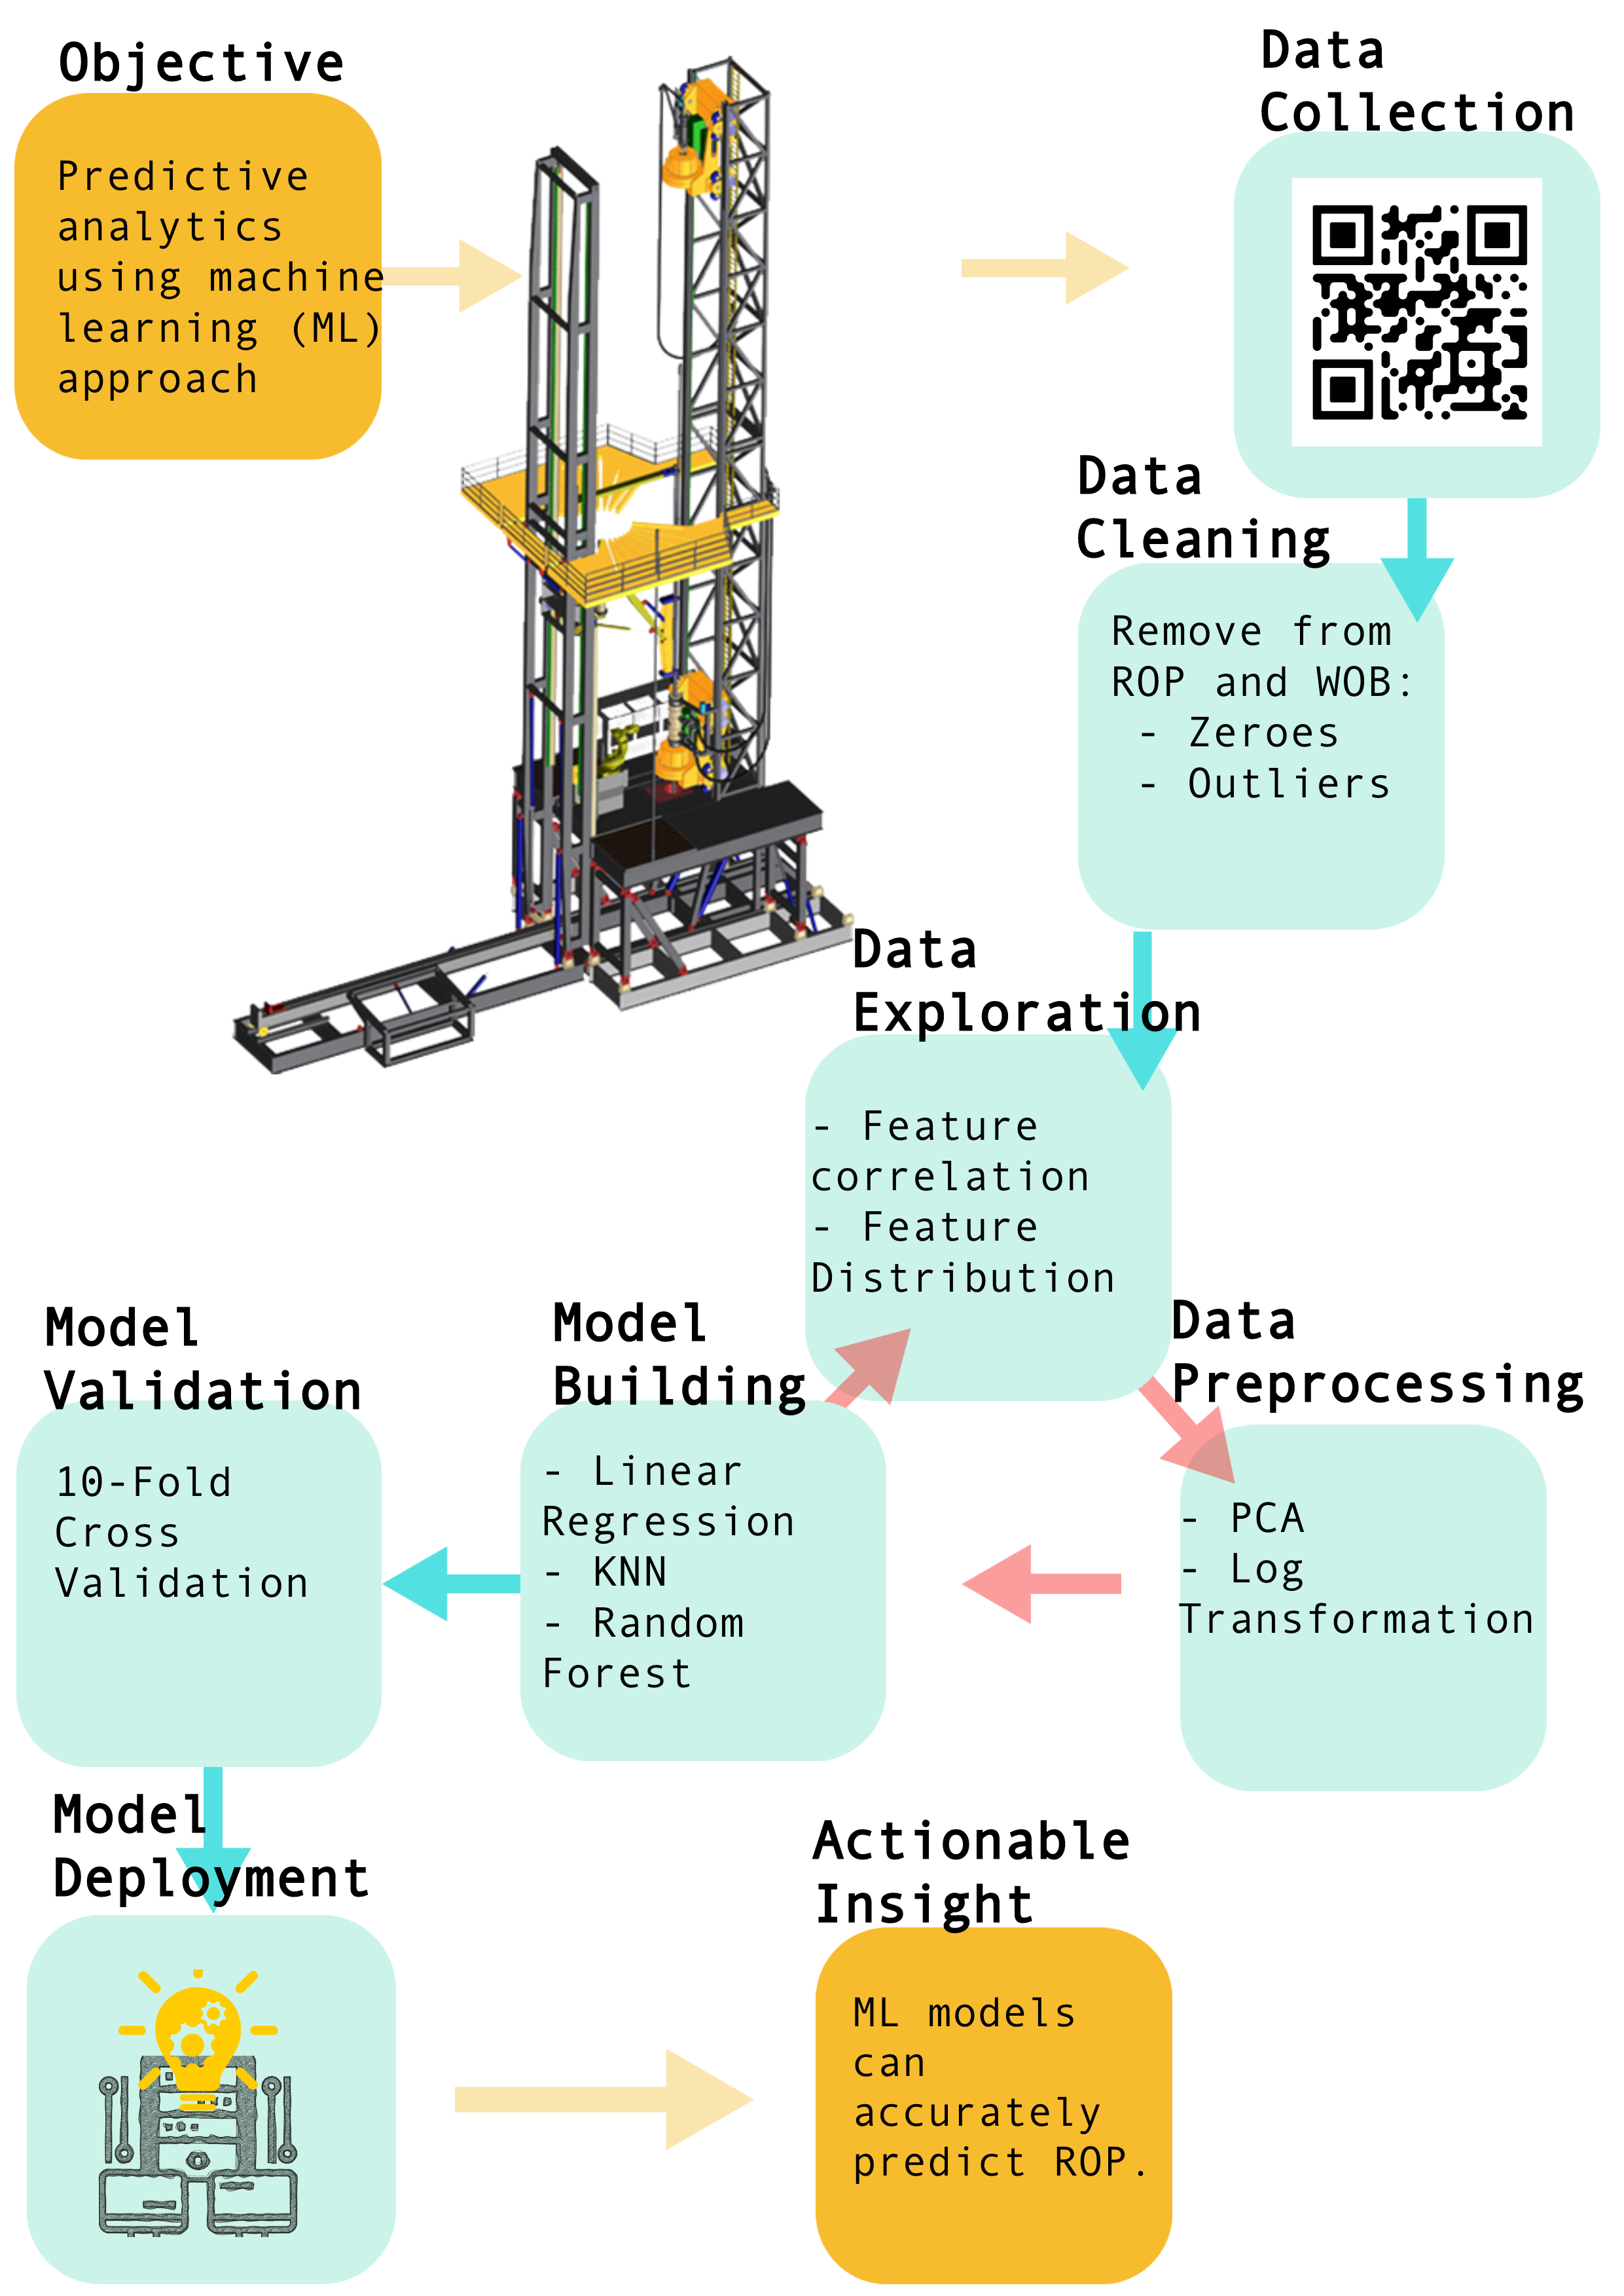
\includegraphics[width=1\textwidth, height = 1.2\textwidth, scale=.70]{Poster/images/Datapipelineproject.png}
    \end{flushright}
%\end{minipage}
  
%\vspace{.50cm}
%\fcolorbox{black}{salmon}
%\begin{minipage}[t]{.96\linewidth}
\vspace{-1cm}
\begin{center}
\section*{Results}    
\end{center}
\vspace{-.25cm}
{\large After evaluating several machine learning models on our dataset, we have identified $\color{red}Random Forest$ as the best model for our dataset. This model achieved the highest R2 score of $\color{red}0.9358$ and the lowest RMSE of $\color{red}0.2320$. Random Forest is an ensemble learning method that uses multiple decision trees to make predictions, which results in a more accurate and stable model compared to other models. In our case, we used $\color{red}200$ trees with the Gini impurity criterion. We recommend using this model for future predictions on our dataset.  }
\end{minipage}
%}
  
% ---------------------------------------------------------------------------

\vspace{.5cm}

%%{\textcolor{rojo}{Something here for aesthetics?}  }


\begin{minipage}[t]{.96\linewidth}
\begin{center}
\noindent
\vspace{-.55cm}
\section*{Model Evaluation}
\end{center}

\begin{center}
\begin{minipage}{.48\linewidth}
  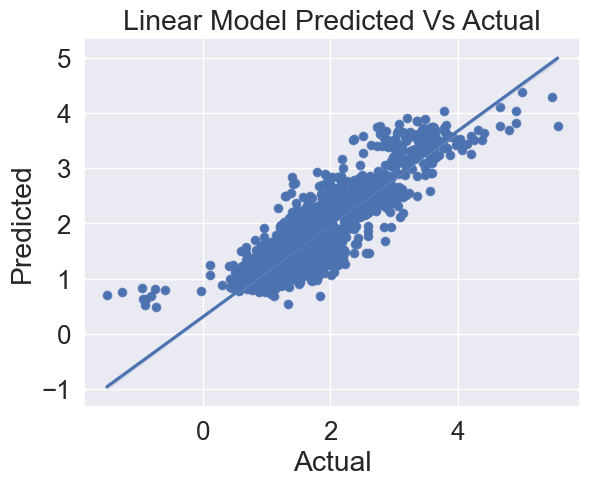
\includegraphics[width=1\linewidth, height=0.9\textwidth, scale=1]{Poster/images/point7.png}
\end{minipage}
\begin{minipage}{.48\linewidth}
  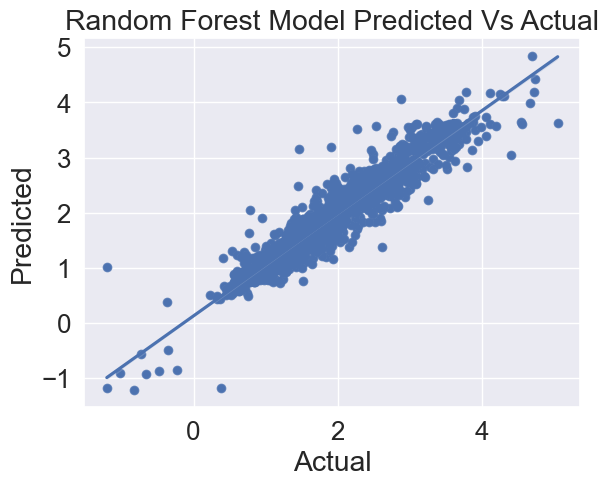
\includegraphics[width=1\linewidth, height=0.9\textwidth, scale=1]{Poster/images/rfPredicted.png}
\end{minipage}  
\end{center}
%\end{minipage}

%\begin{minipage}[t]{.90\linewidth}
    %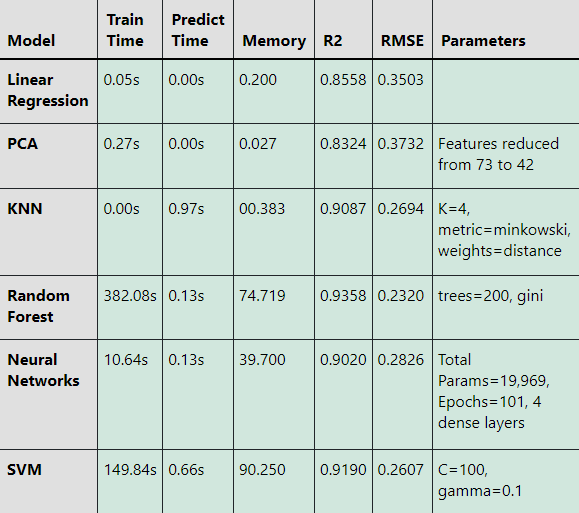
\includegraphics{Poster/images/trainScores.png}
\begin{minipage}[t]{.96\linewidth}
\begin{center}
    
\begin{center}
\noindent
\vspace{-.55cm}
\section*{Results Summary}
\end{center}

    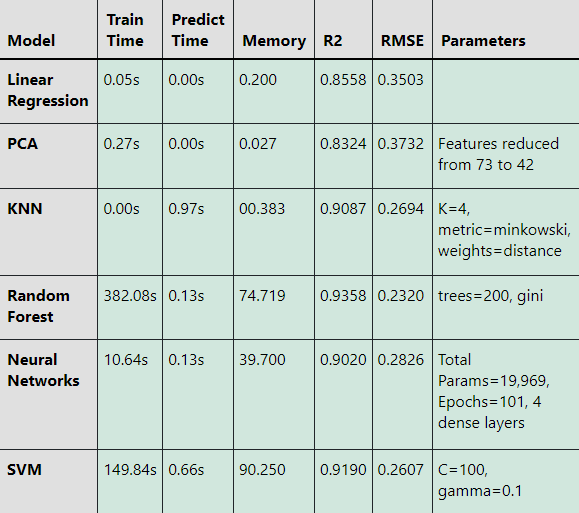
\includegraphics[width=0.9\textwidth, height=.53\textwidth, scale=.65]{Poster/images/trainScores.png}
    %\captionsetup{labelformat=empty}
\end{center}
    \begin{minipage}[t]{.80\linewidth}
    {\small Processor:  Intel(R) Core(TM) i5-9600K CPU @ 3.70GHz 3.70 GHz\\Installed RAM: 16.0 GB\\System type: 64-bit operating system, x64-based processor}
    \end{minipage}
\end{minipage}

\vspace{1.2cm}
%\colorbox{marronrp3}{
    \vspace{.2cm}
  \begin{minipage}[t]{.96\linewidth}
    \begin{center}
    \section*{Conclusion \& Future Work}
    \end{center}
   {\large Random forest produced results with the least amount of errors out of every model utilized. One feature to be incorporated for future work would be depth when dealing with data from more than one oil well. The model could then be better utilized for predictions on larger data sets from multiple oil well sources.} 
   \vspace{.05cm} 
%  \end{minipage}
%}

\vspace{.4cm}
%%\noindent
%%\colorbox{marronrp3}{
%% \begin{minipage}[t]{.96\linewidth}
%%\vspace{.05cm}
%%\begin{center}
%%  \section*{}
%%  \dots
%%\hspace{.15cm}
%%\end{center}
%%\end{minipage} 
%%}

%\begin{minipage}[t]{.90\linewidth}
\noindent
\begin{center}
\bibliographystyle{plain} % We choose the "plain" reference style
\bibliography{refs} % Entries are in the refs.bib file
\end{center}
\end{minipage}
\end{minipage}

\end{multicols}

 \vspace{-1.25cm}
\begin{minipage}[t]{.9756\linewidth}
\begin{center}
\noindent
\section*{Acknowledgements}
\vspace{-.45cm}
This material is based upon work supported by the National Science Foundation under Grants numbers NSF IIS-2123247.
Any opinions, findings, and conclusions or recommendations expressed in this material are those of the authors and do not necessarily
reflect the views of the National Science Foundation.
\end{center}
\end{minipage}

\end{document}

